\chapter{Implementation}

In order to verify the concepts, a prototype was built very early before building the
final system.

\section{Hardware Prototype PCBs}

\begin{figure}[H]
\centering
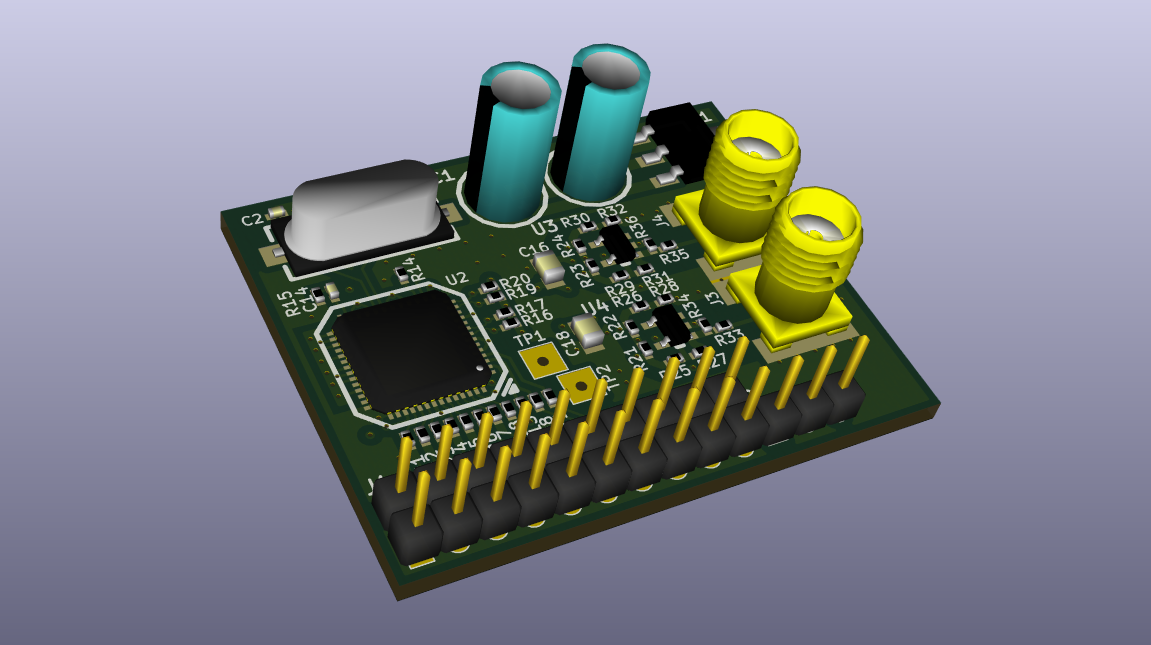
\includegraphics[width=4in]{synth3d.png}
\caption{Synthesizer PCB, 3D render}
\label{fig:synth3d}
\end{figure}

\autoref{fig:synth3d} shows the synthesizer prototype. This contains the \texttt{AD9958} DDS
and its associated support circuitry. A 10~ppm quartz crystal~\cite{txc-9c} was selected
as the frequency response, and testing showed that the frequency stability of the \texttt{AD9958}'s
internal PLL (which was necessary to derive a 500~MHz clock from the 25~MHz crystal) was
sufficient for the accuracy we required.

This board also contained the differential amplifiers, as the output circuit of the
\texttt{AD9958} is inconvenient to connect via external cables. Texas Instruments' inexpensive
\texttt{LMH6714} 400~MHz~\cite{lmh6714} video amplifier was used.

This design worked exactly as expected, and the circuit on this board was carried through to the
final build with no modification.

\begin{figure}[H]
\centering
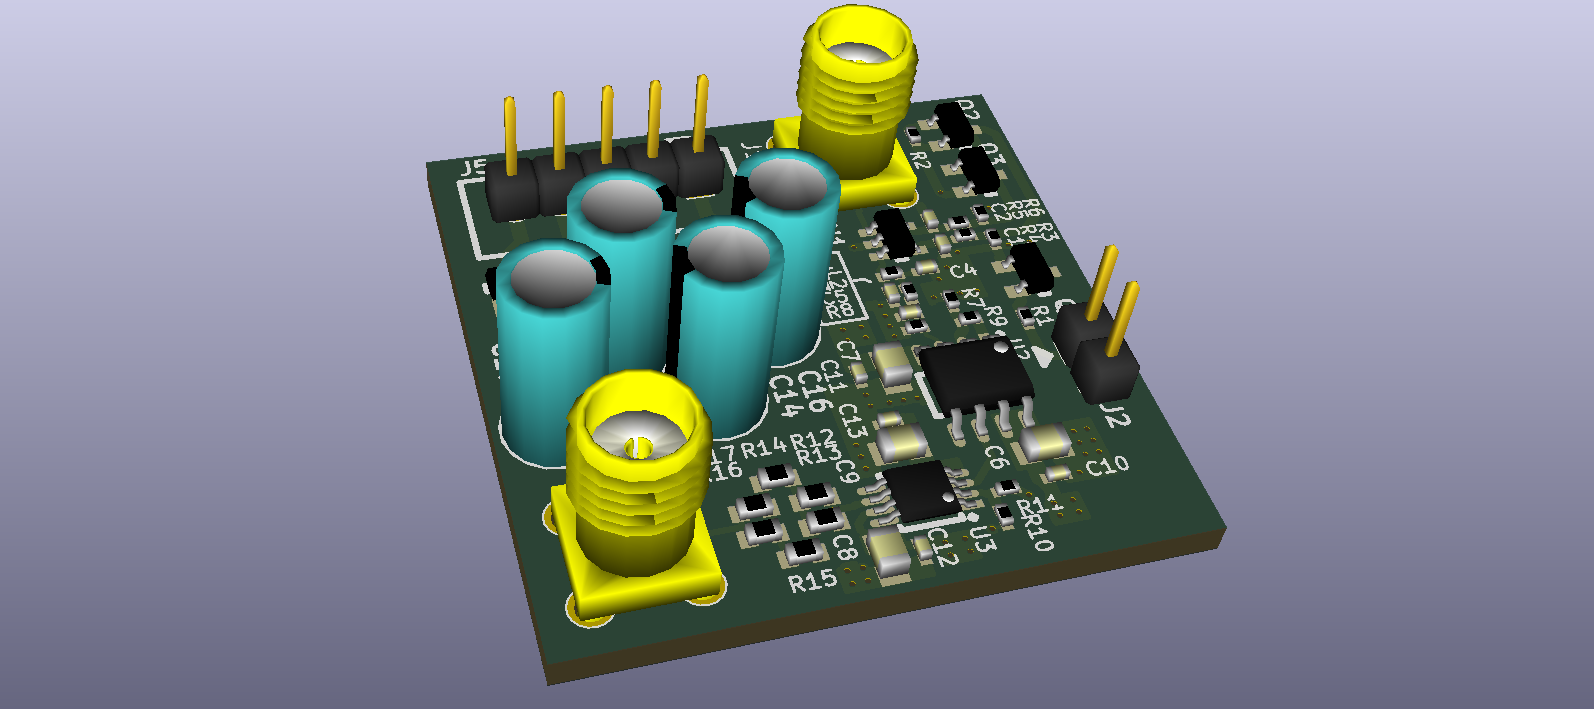
\includegraphics[width=4in]{outamp3d.png}
\caption{Output Amplifier PCB, 3D render}
\label{fig:outamp3d}
\end{figure}

\autoref{fig:outamp3d} shows the output amplifier prototype. This prototype board accepts
the signal directly from the synthesizer. The signal passes through a \texttt{MAADSS0008}
switched 15\;dB attenuator, through a fifth-order Butterworth low-pass filter, and into
the amplifiers. Testing revealed two problems with this design, both caused by the low-pass
filter. The gradual roll-off of the fifth-order filter meant that the filter was both
inadequate at removing all Nyquist aliases, and had too much loss at the high end of the
desired passband.

For the final build, a precision, seventh-order elliptical filter was used. This filter
design was prototyped and tested on its own, to verify that it would have the desired
cutoff properties; it passed this test and so was used in the final design. No other
changes were made here.

\begin{figure}[H]
\centering
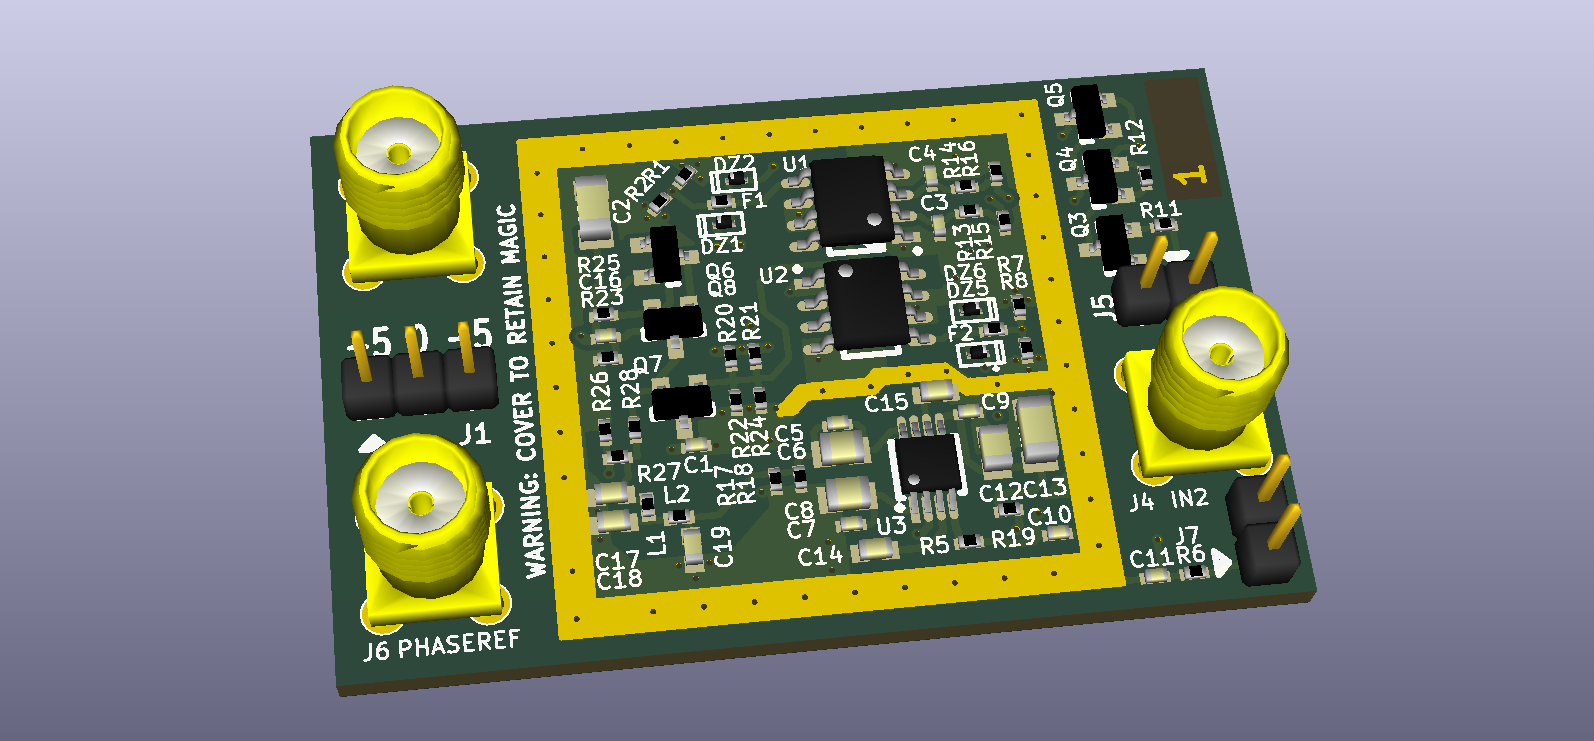
\includegraphics[width=4in]{frontend3d.png}
\caption{Input Front-end PCB, 3D render}
\label{fig:front3d}
\end{figure}

\autoref{fig:frontend3d} shows the input frontend prototype. This contains the input
protection network, the switches, the buffer, the filter, and the logarithmic detector.
It has two coaxial inputs for the primary input signals, and one to be directly fed the
phase reference signal from the synthesizer. This design also worked exactly as intended.
The circuit was kept unchanged, though the layout was redone to fit the overall layout of
the final board.

\section{Microprocessor Software Prototyping}

To prototype the microprocessor software, a development board was used rather than
designing a custom PCB. An Atmel `SAM4S Xplained' board, which holds a \texttt{SAM4S16C}
(the largest member of the SAM4S series), an SRAM module, and an on-board programmer, was
connected to the prototype boards. The final firmware was small, so the smaller but otherwise
identical \texttt{SAM4S4C} was used in the final build.

\section{PC Software}

PC software was developed using Python. The TkInter graphical user interface toolkit was
used to build the application, `matplotlib' (a plotting library) was used to draw plots,
and pySerial was used to provide communcations with the instrument.
